\documentclass[conference]{IEEEtran}
\usepackage{times}
\usepackage[numbers]{natbib}
\usepackage{amsmath,amssymb,booktabs,graphicx}
\usepackage[bookmarks=true]{hyperref}
\hypersetup{hidelinks,pdfauthor={},pdftitle={The Cost of Certifying VLA Updates under Statewise Regression Budgets},
 pdfsubject={Finite-suite decision methods and development experiments},pdfkeywords={}}
\begin{document}
\title{The Cost of Certifying VLA Updates\\under Statewise Regression Budgets}
\author{Author Names Omitted for Anonymous Review}
\maketitle
\begin{abstract}

An increase in aggregate task success does not establish that a policy update preserves previously successful states. We study a finite-suite decision objective that budgets the weighted positive part of statewise success loss, rather than allowing gains elsewhere to cancel regressions. Applying standard mixture confidence sequences to paired discordance indicators gives an anytime-valid accept, reject or uncertain decision. A pooled-discordance sufficient gate provides a necessary simple baseline, alongside marginal and joint statewise bounds with uniform or adaptive allocation and a terminal exact method. In a fresh development cohort of eight synthetic scenarios with 20 states and 30 repetitions each, the pooled gate admits every low-disagreement and improved run at median costs of 510 and 740 pairs, while statewise methods spend substantially more. When aggregate success improves despite concentrated losses, the pooled gate is always uncertain; joint adaptive profiling rejects every run at a median of 620 pairs. All methods remain uncertain near the budget. Historical five-repeat statewise replay is also inconclusive. The findings distinguish cheap sufficient decisions from cases requiring statewise evidence and motivate a bounded, explicitly specified two-family closed-loop study. They establish neither new statistical theory nor a universal certification-cost lower bound.

\end{abstract}\IEEEpeerreviewmaketitle
\section{Motivation and scope}

VLA updates may change precision, inference steps or policy implementation. Aggregate comparisons can conceal a loss on some initial states. The prior workshop paper \emph{Higher Success, New Failures: Measuring Per-State Regressions in VLA Policy Updates} \cite{prior} documents that evaluation problem. The question here is different: what statistical evidence would justify admitting an update under a declared regression budget, and how much evaluation would it cost?

A test that fails to detect a regression need not demonstrate a sufficiently small regression. Conversely, conservative simultaneous state profiling may spend far more than a sufficient aggregate gate. A practical procedure must first ask whether statewise evidence is needed, allow an uncertain outcome, compare against fixed-horizon alternatives, and disclose what it does not cover.

This note supplies an explicit finite-suite objective, a conservative standard confidence-sequence construction, and a reproducible development assessment. The statistical construction is not new theory. The preliminary empirical contribution is the joint picture of allocation benefits and certificate cost. Whether those observations persist on new closed-loop VLA data remains open.

\section{Relation to prior work}

STEP \cite{step} studies sequential robot-policy comparison with near-optimal stopping. SAVI-based policy comparison \cite{savi} extends rigorous sequential comparison to richer performance metrics. Sequential evaluation and rollout savings are therefore established ideas. Our proposed question concerns a nonlinear, statewise regression-loss objective and its admission cost, rather than claiming sequential testing itself as a contribution.

Admission \cite{admission} audits how update gates affect continual embodied learning. It already analyzes rule-specific unchanged-behavior certification cost, repairs a range-based gate with paired-binomial intervals, and reports missed learning opportunities under fixed budgets. Those observations are not contributions claimed here. Its contract is a conjunction of taskwise retention and gain constraints with historical references; our question uses a weighted positive-part statewise budget and asks when pooled sufficient evidence can replace state profiling. A complete paper still needs useful allocation behavior and new closed-loop evidence beyond this simulation. Compressed-policy collapse \cite{collapse} demonstrates why offline checks can fail to predict execution. Benchmark bugs and design limitations \cite{bugs} further show that measured acceleration gains may be evaluator artifacts. Consequently, benchmark reset and success-checker audits are prerequisites for the next phase.

VLAQuantBench \cite{quantbench} already studies closed-loop quantization across four policies, numerical recipes and component scopes, with separate hardware measurements. Its released records and same-observation replay show that quantization failure and recipe dependence are established topics. Our simulated weight-rounding controls therefore supply update cases rather than a new quantizer or acceleration result. The prospective evaluator must bind executed action count, simulator version and actual hook coverage explicitly.

Compatibility-aware classification already separates overall performance from new errors on previously correct inputs \cite{backward}. With deterministic outcomes and $\delta$=0, our objective reduces to a weighted harmful-flip rate. With stochastic outcomes, it uses marginal success loss rather than $q_+$ alone: gains within a state can offset harmful discordance at that state, while gains at other states cannot. It therefore does not promise that every individually successful rollout is preserved. Backward compatibility and statewise loss are established concerns; the proposed contribution is a measured decision-cost study for the stated finite-suite objective.

\section{Decision objective and certificate}

Fix S states and nonnegative weights $w_s$ summing to one before observing evaluation outcomes. Pair old and new binary success outcomes within each fresh repeat. Define

\begin{align}
D_s&=X_{\mathrm{old},s}-X_{\mathrm{new},s}\in\{-1,0,1\},\\
q_{+,s}&=\Pr(D_s=1),\quad q_{-,s}=\Pr(D_s=-1).
\end{align}

The marginal success difference is $q_{+,s}-q_{-,s}$. Dependence within an old/new pair does not change this identity. For tolerance $\delta$ and budget $\epsilon$, the objective is

\begin{equation}
R_\delta=\sum_s w_s\max(q_{+,s}-q_{-,s}-\delta,0)\leq\epsilon.
\end{equation}

Improvements at other states do not cancel the positive losses. This is a weighted aggregate of statewise excess losses, however, not a requirement that every state avoid harm. For equal weights, one severely harmed state may still fit the total budget. The choice of weights and thresholds must reflect the actual deployment objective.

For each positive or negative discordance indicator, let n be its observation count and k its count of ones. Use the standard Jeffreys mixture process, within the established confidence-sequence framework \cite{howard}:

\begin{equation}
E_n(p)=\frac{B(k+1/2,n-k+1/2)}
 {B(1/2,1/2)p^k(1-p)^{n-k}}.
\end{equation}

Invert $E_n(p)$ $<$ 1/a with a = $\alpha$/(2S) to obtain confidence intervals for the 2S indicator probabilities. Ville's inequality and a union bound yield simultaneous coverage over states and all sample sizes. From interval endpoints $[l_+,u_+]$ and $[l_-,u_-]$, form

\begin{align}
L&=\sum_s w_s\max(l_{+,s}-u_{-,s}-\delta,0),\\
U&=\sum_s w_s\max(u_{+,s}-l_{-,s}-\delta,0).
\end{align}

Accept when U $\leq$ $\epsilon$; reject when L $>$ $\epsilon$; otherwise collect more data or return uncertain at the cap. For one predeclared update, the probability of any wrong decision is at most $\alpha$, under the assumptions below. This follows from the simultaneous coverage event, not from a zero-error simulation count. The mixture and its assumptions are specified above; the categorical comparator is specified below.

Each state's fresh repeat must retain its fixed conditional discordance probabilities given the observed past. The allocation must be predictable. Serial dependence or probability drift violating that condition is outside the guarantee. The suite must be predeclared; the result does not certify unseen tasks. Searching multiple updates also requires a family error allocation.

We compare uniform allocation with a heuristic selecting the largest current weighted loss-interval width. The heuristic sees only past outcomes and has no optimality guarantee. Both methods share the same certificate. The terminal baseline uses exact binomial intervals with the same state/indicator error allocation and one end-of-budget inspection; it is not valid for repeatedly peeking at intermediate terminal intervals.

\subsection{A pooled-discordance sufficient gate}

Draw each state independently with the declared weights and collect one fresh pair. Let h and g be the weighted average harmful and beneficial discordance probabilities. Jensen's inequality and the pointwise bound $\max(q_+-q_--\delta,0)$ $\leq$ (1-$\delta$)$q_+$ give

\begin{equation}
\max(h-g-\delta,0)\leq R_\delta\leq (1-\delta)h.
\end{equation}

Thus pooled Bernoulli mixtures with $\alpha$/2 for each indicator give

\begin{equation}
L=\max(l_h-u_g-\delta,0),\quad U=(1-\delta)u_h.
\end{equation}

The same decision rule has the same $\alpha$ wrong-decision guarantee.

This sufficient gate can avoid state profiling when discordance is rare. Its lower bound can also reject large average losses. It cannot in general recover the nonlinear statewise objective: compensation across states can make its lower bound uninformative even when $R_\delta$ exceeds the budget. The pooled Bernoulli inference requires IID state draws and fresh conditional outcomes. It does not apply unchanged to adaptive sampling or deterministic cycling. Method comparisons use $\alpha$ individually; selecting the first decision across gates requires a separate error split. State switching may also increase real execution cost.


\begin{figure*}[t]
\centering
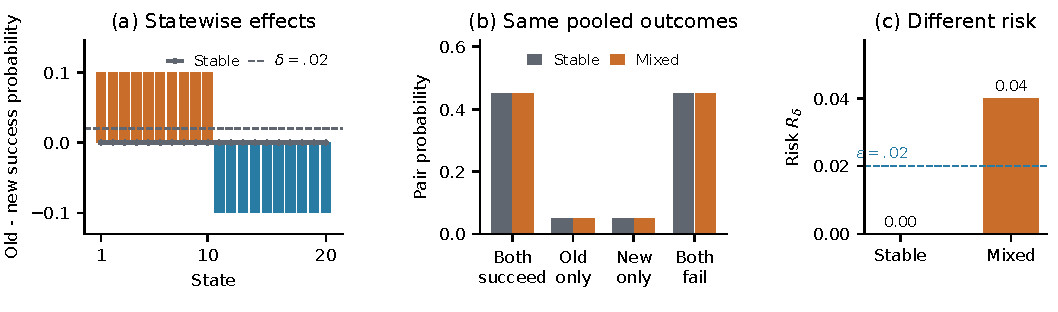
\includegraphics[width=\textwidth]{aggregate-identifiability.pdf}
\caption{Exact analytic construction, not sampled trials or VLA outcomes.
Twenty equally weighted states have the same pooled old/new success rates
(both .50) and the same pooled paired-outcome law in two suites. Their
statewise risks are 0 and .04 at $\delta=.02$, on opposite sides of
$\epsilon=.02$. Discarding state identities prevents general identification
of this nonlinear objective, even when the pooled law is known exactly.
This does not imply that every state needs a tight separate interval.}
\label{fig:identifiability}
\end{figure*}



\subsection{Self-contained joint-region specification}
For counts $b,c,z$ of positive, negative and zero discordance, $n=b+c+z$.
The Dirichlet mixture likelihood is
\begin{equation}
M_n=\frac{\Gamma(3/2)}{\Gamma(n+3/2)}
 \prod_{k\in\{b,c,z\}}\frac{\Gamma(k+1/2)}{\Gamma(1/2)}.
\end{equation}
Invert $M_n/(q_+^b q_-^c q_0^z)\leq S/\alpha$ on the simplex
$q_++q_-+q_0=1$. Ville's inequality and a statewise union bound cover
all states and inspection times under the same fresh-repeat assumptions.
Project each covered region onto $d=q_+-q_-$ and aggregate the resulting
endpoints by the same monotone loss function. This preserves the stated
wrong-decision bound.

The projection profiles the categorical likelihood over
$t=q_++q_-\in[|d|,1]$, with $q_+=(t+d)/2$, $q_-=(t-d)/2$ and $q_0=1-t$.
Check feasible endpoints and stationary roots of
\begin{equation}
nt^2-[(b+c)+(b-c)d]t+[(b-c)d-zd^2]=0.
\end{equation}
Log-concavity gives an interval in $d$; outward bisection returns
conservative numerical endpoints. Independent scalar optimization and
a feasible-simplex grid check the implementation. At support boundaries
the mixture process is a supermartingale on possible sample paths.
No optimality or uniform-tightness claim is made.

\section{Development experiments}

The frozen configuration uses S=20, uniform weights, $\alpha$=.05, $\delta$=.02, $\epsilon$=.02, batches of ten pairs and a cap of 5,000 pairs per strategy. Each pair corresponds to two policy episodes. Seven synthetic discordance distributions cover unchanged low-disagreement outcomes, improvement, diffuse harm, losses just inside/outside the budget, sparse severe harm and heterogeneous harm. These are constructed stress distributions, not fitted robot populations. The label "unchanged" means equal old/new success probabilities; its small nonzero discordances do not represent bit-identical execution of the same deterministic pipeline with the same random stream.

Earlier development cohorts compared marginal, joint and terminal methods. A concern about deterministic tie breaking prompted an independent seed and randomized harmed-state locations before the second cohort. Those records are preserved; the fresh six-method comparison below includes the missing pooled gate and compensated-loss control. These are development experiments, not held-out robot studies.

\subsection{Fresh six-method comparison with a simple sufficient gate}

The final development amendment was frozen before collecting a fresh seed. It adds the pooled gate and a compensated-loss scenario to the earlier seven cases. There are 30 independent repetitions per case, with random state locations and six paired strategies sharing each repetition's state streams: 1,440 strategy rows from 240 independent scenario repetitions. Parameters and the 5,000-pair cap are unchanged. The pooled method uses an independent uniform state draw for every pair, inspecting after every ten observations.

The compensated case sets $q_+$=.35,$q_-$=0 on five states and $q_+$=0,$q_-$=.13 on fifteen. Aggregate success improves by .01, while $R_\delta$=.0825 exceeds .02. This constructed case isolates cross-state compensation; it is not evidence that natural VLA updates have that distribution.

Figure~\ref{fig:identifiability} separately illustrates the identifiability limitation with an exact constructed pair of suites. This is an analytic example, separate from the sampled development experiment.

Each cell reports verdict counts out of 30 followed by median pairs consumed. A, R and U denote accept, reject and uncertain. The median includes runs censored at the cap and is not necessarily a median time to a decision.

\begin{table*}[t]\centering\caption{Fresh six-method development cohort: verdict counts out of 30; median consumed pairs, including uncertain runs at the cap.}\small
\begin{tabular}{lcccccc}\toprule
Scenario & Marg. uniform & Marg. adaptive & Joint uniform & Joint adaptive & Terminal & Pooled IID \\
\midrule
Unchanged & 30U; 5,000 & 30U; 5,000 & 30U; 5,000 & 30U; 5,000 & 30A; 5,000 & 30A; 510 \\
Improved & 24A/6U; 4,795 & 27A/3U; 4,740 & 30A; 3,485 & 30A; 3,350 & 30A; 5,000 & 30A; 740 \\
Diffuse harm & 30U; 5,000 & 30U; 5,000 & 30U; 5,000 & 30U; 5,000 & 30U; 5,000 & 30R; 1,620 \\
Inside budget & 30U; 5,000 & 30U; 5,000 & 30U; 5,000 & 30U; 5,000 & 30U; 5,000 & 30U; 5,000 \\
Outside budget & 30U; 5,000 & 30U; 5,000 & 30U; 5,000 & 30U; 5,000 & 30U; 5,000 & 30U; 5,000 \\
Sparse harm & 30R; 1,990 & 30R; 565 & 30R; 1,355 & 30R; 330 & 30R; 5,000 & 7R/23U; 5,000 \\
Heterogeneous & 30R; 3,020 & 30R; 915 & 30R; 1,875 & 30R; 700 & 30R; 5,000 & 1R/29U; 5,000 \\
Compensated & 30R; 2,270 & 30R; 885 & 30R; 1,500 & 30R; 620 & 30R; 5,000 & 30U; 5,000 \\
\bottomrule\end{tabular}
\end{table*}

The pooled baseline wins decisively in the low-disagreement, improved and diffuse-harm cases; reporting only its failures would misrepresent the evidence. Statewise profiling wins in concentrated and compensated-loss cases. The compensated result supports investigating the nonlinear objective rather than asserting that all acceptance requires exhaustive profiling. No method resolves either near-budget case. There are no observed wrong decisions. For one independent 30-repetition scenario/strategy cell, the two-sided exact 95\% upper error endpoint is 11.57\%; paired strategy rows do not increase the independent denominator.

The audit reconstructs consumed state streams, verifies IID state-prefix counts and first inspected stopping times, and independently inverts the Bernoulli mixtures using SciPy roots. It also checks archived source hashes, final bounds, decisions and all 48 summary cells. Full records are in the archived verified analysis.

\subsection{Descriptive historical replay}

We paired 500 existing old/new observations for each of four updates across 100 fixed states. Pair identity includes task, initial state, scene seed, repeat and policy seed; duplicates and incomplete matches are rejected.

\begin{table*}[t]\centering\caption{Descriptive replay of historical five-repeat records; not true-risk estimates.}\small
\begin{tabular}{lccc}\toprule
Historical update & Plug-in R & Certificate interval & Verdict \\
\midrule
BF16 & .0344 & [0, .8464] & Uncertain \\
W4 weight-rounding experiment & .0168 & [0, .8449] & Uncertain \\
W3 weight-rounding experiment & .2014 & [0, .8794] & Uncertain \\
Two inference steps & .0036 & [0, .8407] & Uncertain \\
\bottomrule\end{tabular}
\end{table*}

These historical data have five repeats per state. The plug-in risks are noisy positive-part estimates, not true risks. Complete pairing does not establish the fresh-repeat assumptions, evaluator correctness or freedom from selection. Thus this replay is descriptive and cannot validate a newly tuned online allocation rule. Weight rounding is also not genuine integer-kernel execution.

\section{Certificate cost and implications}

For the implemented bounds, one can deterministically find the equal number of repeats needed when \textbf{every observed pair has zero discordance}. With 100 states and the stated thresholds, the anytime construction first admits at 287 repeats per state: 28,700 pairs or 57,400 policy episodes. The terminal exact construction requires 221 repeats per state.

This calculation characterizes these particular conservative bounds under balanced sampling. It is not an information-theoretic lower bound, an expected rollout cost, or a claim that all better procedures need that many episodes. It explains the inconclusiveness of the historical statewise replay; it does not establish that every valid gate needs comparable data. The joint construction is worse in this particular zero-observed-discordance calculation: it requires 347 repeats per state for 100 states, or 34,700 pairs. For 20 states it requires 304 repeats versus the marginal construction's 246. The joint endpoint in this case is exactly $1-[\alpha/(S(2n+1))]^{1/n}$; an independent closed-form calculation checks the numerical projection. A dimensionality penalty can outweigh the benefit of modeling the indicators jointly. Neither construction is a universal lower bound. The next study must measure actual rollout and policy-switching costs.

Under IID state sampling, the pooled gate instead first admits all-zero discordance at 349 total pairs, or 350 at ten-pair inspections, independent of the suite size. This is an observed-data calculation for that bound, not an expected cost or a guarantee that discordances stay zero. It directly prevents treating the 28,700 or 34,700 statewise counts as a general cost of the regression objective.

The study must distinguish cheap sufficient decisions from cases requiring statewise evidence. It does not support the claim that anytime certification is generally cheaper than terminal tests. Rejection can follow from a large loss on a few states or a sufficient average loss. Acceptance can follow from a sufficiently small pooled harmful-discordance rate; full state profiling is not always necessary.

\section{Testable hypotheses and next study}

The development evidence motivates three hypotheses; it does not confirm them on new VLA outcomes:

\begin{enumerate}
\item For losses concentrated on a few states and separated from the declared
budget, predictable width allocation reduces paired correct-rejection cost
relative to uniform allocation using the same certificate.
\item A joint categorical certificate improves decisiveness in some mixed-
discordance regimes, but does not uniformly improve acceptance cost when
discordances are rare.
\item A pooled-discordance sufficient gate avoids costly state profiling when
discordance is rare, but compensated losses require statewise evidence.
Under a finite cap, an uncertain result may remain the correct conclusion.

\end{enumerate}
Before the new cohort, operationalize concentration and separation using a separate reference cohort with intervals, freeze effect-size thresholds, and declare how inconclusive reference cases will be handled. Do not choose those thresholds after seeing the tested methods' costs. If no genuine update supplies the intended sparse-loss regime, report that coverage gap instead of treating the deliberately harmful stress control as natural policy evidence.

Before a full archival final submission, collect fresh closed-loop data from at least two VLA families and updates declared before observing outcomes. Use an independent suite, fresh paired randomization, reset/success-checker audits, all-attempt logging and a separately declared reference-risk cohort with uncertainty. Begin with a bounded pilot; do not launch tens of thousands of rollouts simply to satisfy the present conservative interval.

The study must compare matched uniform/adaptive procedures, a terminal exact baseline, the joint certificate and the pooled sufficient gate. Report accepts, rejects and uncertain outcomes, cost distributions, family error accounting and measured execution overhead. The experiment remains prospective; a full final paper requires substantive new validation.

\subsection{Operational design for the prospective bounded pilot}

The planned families are X-VLA and $\pi_{0.5}$ using pinned public LIBERO checkpoints. Model-health checks use five separately declared states and a fixed gate of at least three successes with no infrastructure or reset error. Failure to pass this gate is a feasibility result; it does not authorize replacing a family after seeing update outcomes. Checkpoint precision is FP32 for X-VLA and BF16 for $\pi_{0.5}$, with the official selective FP32 components. Preserve the official processors, including normalization statistics. Record predicted and executed action counts separately; the pinned PI05 configuration executes 50 actions per prediction. This defines our checkpoint-default pipeline, not a reproduction of other clients that execute ten actions.

Select two states per LIBERO-10 task from indices 20--49, excluding every local pilot and health-check state, using seed 2026093007 before update outcomes. Verify the actual candidate inventory and initial-state file hashes before freezing the suite. Uniform weights define a 20-state target. Scene identities remain fixed; fresh paired policy seeds are drawn from a separate reproducible stream.

For each family declare four comparisons: independently reload the identical pipeline; simulated group-128 four-bit rounding of linear weights; group-128 three-bit rounding as a severe stress control; and two instead of ten flow steps. Preserve checkpoint precision, action transforms and the 520-step horizon otherwise. X-VLA uses absolute control and $\pi_{0.5}$ relative control. Stress controls are reported separately from practically motivated updates. Neither weight rounding nor a shared-GPU run supports a hardware speed claim.

Use $\alpha_{\mathrm{total}}$=.05 across eight comparisons and six methods, allocating .05/(8*6) to each method/update. Report .05/8 as a separately labelled per-method-family sensitivity analysis, without a combined-gate claim. Each strategy has a 1,000-pair cap with ten-pair batches and may return uncertain. Compare both marginal and joint certificates with uniform and adaptive allocation, a single-inspection terminal exact method, and a pooled gate using independently drawn uniform states per pair. Share recorded per-state streams only through a cache whose outcome access is restricted to each strategy's consumed prefix. Collect missing pairs on demand; the actual union of collected pairs may exceed any one strategy's cap. Report both the virtual consumption of each method and all physical episodes needed for the comparison. Also record resets, processor time, checkpoint switching and errors.

A separate fixed reference cohort has 50 fresh pairs per state. Exact simultaneous intervals with a separate .05 family budget describe its risk uncertainty; this is not an additional source of decision validity. Label realized wrong decisions only when the reference interval is wholly on one side of $\epsilon$. Otherwise report the reference as inconclusive. Never use the noisy positive-part point estimate as true risk.

For allocation assessment, report per-update paired savings when both methods reject and the reference interval supports rejection. Predeclare 25\% savings as a practically useful target. Describe concentration using the independent reference estimate and its interval; if no natural update supports the intended concentrated-loss regime, disclose that coverage gap. Eight comparisons from two families do not support broad population inference. A first 12 GPU-hour feasibility cap precedes expansion based on measured execution cost. Unexecuted comparisons and infrastructure failures are distinct from statistical uncertainty at a fully consumed cap. All protocol revisions precede their new cohorts.


\section{Reproducibility and limitations}

The run directories preserve source snapshots, pre-collection manifests, seeds, outcome summaries and per-repetition counts. An analysis script reconstructs consumed synthetic outcomes and checks recorded bounds and decisions. Frozen methods and outcome archives are distinct from later analysis and document-generation code.

The update study has no new robot outcome cohort, no hardware safety guarantee, no cross-model result, and no demonstrated generalization outside its declared suite. LIBERO-MAX \cite{max} is a new adjacent paired-event benchmark; pairing by itself is not a contribution. Its environment-event objective differs from the finite-suite policy-update decision objective studied here. The new paper's contribution must come from its decision objective, measured cost regimes and substantive validation. The current draft specifies and assesses that direction.

\clearpage
\bibliographystyle{plainnat}
\bibliography{references}
\end{document}
